\documentclass[12pt]{article}
\usepackage[utf8]{inputenc}
\usepackage{graphicx}
\usepackage{listings}

\title{Analysis and Design of Algorithms}
\author{}
\date{April 2019}

\usepackage{natbib}
\usepackage{graphicx}
\usepackage{hyperref}

\begin{document}

\maketitle

Name : Jonathan Loza Mendoza\\
\section{Warm up}

Lets modify the classic merge sort algorithm a little bit. What happens if instead of splitting the array in 2 parts we divide it in 3? You can assume that exists a three-way merge subroutine. What is the overall asymptotic running time of this algorithm?

\emph{BONUS:} Implement the three-way merge sort algorithm.\\

    \\Rpta:\\
    If we split the array in 3 parts the recursive tree may reduce its height. Now that the array subdivide in 3 parts the T(n) will be equal to 3T(n/3) + n instead of the 2T(n/2)+n. The overrall asymptotic running time may be :\\
  \\$ {\Theta(n\log_3 n})$\\
   \\This time the base of the log is 3 instead of base 2 because of the 3 division of n

\section{Competitive programming}

Welcome to your first competitive programming problem!!! 

\begin{itemize}
    \item Sign-up in Uva Online Judge (\url{https://uva.onlinejudge.org}) and in CodeChef if you want (we will use it later).
    \item Rest easy! This is not a contest, it is just an introductory problem. Your first problem is located in the ``Problems Section'' and is \textbf{100 - The 3n + 1 problem}.
    
    \item Once that you finish with that problem continue with \textbf{458 - The Decoder}. Again, this problem is just to build your confidence in competitive programming.
    
    \item \emph{BONUS:} \textbf{10855 - Rotated squares}\\
    
    \begin{lstlisting}[language=C++, caption={The 3n+1 problem}]
#include <iostream>
#include <vector>
#include <string>

using namespace std;

int operation(int a, int b){
  int x;
  int ciclomax=0;
  int ciclo;
  if(a>b){
    x=a;
    a=b;
    b=x;
  }
  for(a;a<=b;a++){
    ciclo=1;
    x=a;
    while(x!=1){
      if(x%2!=0){
        x=3*x+1;
      }
      else{
        x=x/2;
      }
      ciclo+=1;
    }
    if(ciclo>ciclomax){
      ciclomax=ciclo;
    }

  }
  return ciclomax;
}

int main(){
  int x,y;
  while(cin>>x>>y){
    cout<<x<<" "<<y<<" "<<operation(x,y)<<endl;
  }
\end{lstlisting}

\begin{lstlisting}[language=C++, caption={Decoder}]
#include <iostream>
#include <string>

using namespace std;

int main(){
  string str;
  string answer="";
  while(cin>>str){
    int x=str.size();
    for(int i=0;i<x;++i){
      answer+=str[i]-7;
    }
    cout<<answer<<endl;
    answer="";
  }
  return 0;
}

\end{lstlisting}



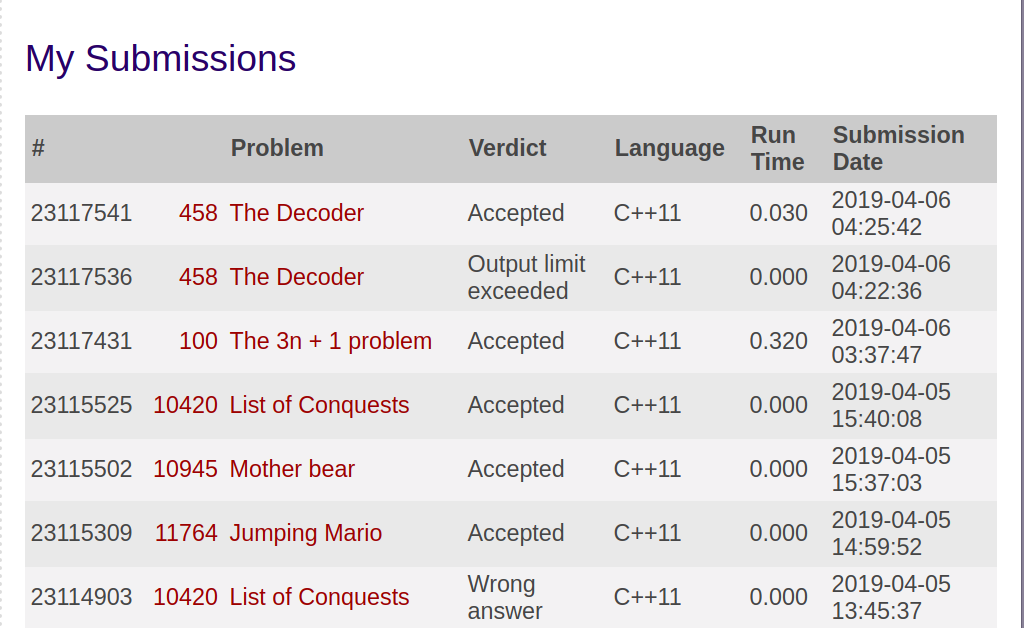
\includegraphics[width=\textwidth]{Src/UVA1.png}

\end{itemize}

\section{Simulation}

Write a program to find the minimum input size for which the merge sort algorithm always beats the insertion sort.

\begin{itemize}
    \item Implement the insertion sort algorithm
    \item Implement the merge sort algorithm
    \item Just compare them? No !!! Run some simulations or tests and find the average input size for which the merge sort is an asymptotically ``better'' sorting algorithm.
\end{itemize}

Note: Include (.tex) and attach(.cpp) your source code and use a dockerfile to interact with python and plot your results.\\

\emph{BONUS:} Compare both algorithms against any other sorting algorithm\\


\begin{lstlisting}[language=C++, caption={Insertion sort vs Merge sort}]
#include <iostream>
#include <vector>
#include <math.h>
#include <fstream>
#include <random>
#include <limits>
using namespace std;
void merge(vector<int>& a,int begin, int medio, int end){

    int n1=medio-begin+1;
    int n2=end-medio;
    vector<int> left;
    vector<int> right;
    for(int i=0;i<n1;++i){
        left.push_back(a[i+begin]);
    }
    for(int j=0;j<n2;++j){
        right.push_back(a[j+medio+1]);
    }
    left.push_back(std::numeric_limits<int>::max());
    right.push_back(std::numeric_limits<int>::max());
    int i=0;
    int j=0;
    for(int k=begin;k<=end;++k){
        if(left[i]<=right[j]){
            a[k]=left[i];
            i++;
        }
        else{
            a[k]=right[j];
            j++;
        }
    }
}

void mergesort(vector<int>& a, int begin, int end){
    if(begin<end){
        int q=(begin+(end-1))/2;
        mergesort(a,begin,q);
        mergesort(a,q+1,end);
        merge(a,begin,q,end);
    }
}


vector<int> insertionsort(vector<int>& a){
    for(int j=1;j<a.size() ;++j){
        int key=a[j];
        int i=j-1;
        while(i>=0 and a[i]>key){
            a[i+1]=a[i];
            i--;
        }
        a[i+1]=key;
    }
    return a;

}

int main() {
    int average;
    ofstream file("data.dat");
    float timeinsert,timemerge;
    int n=600;
    int veces=0;
    vector<int> num;
    vector<int> num1;
    vector<int> num2;
    while(veces<100) {
        srand((unsigned) time(0));
        int randint;
        for (int index = 0; index < n; index++) {
            randint = (rand() % 1000) + 1;
            num.push_back(randint);
        }
        num1 = num;
        num2 = num;
        clock_t start = clock();
        mergesort(num1, 0, num1.size() - 1);
        clock_t time = clock() - start;
        timemerge=static_cast<float>(time) / CLOCKS_PER_SEC;
        cout << "Mergesort = " << timemerge<< endl;
        start = clock();
        num2 = insertionsort(num2);

        time = clock() - start;
        timeinsert=static_cast<float>(time) / CLOCKS_PER_SEC;
        cout << "Insertionsort = " << timeinsert << endl;
        cout<<"Merge"<<endl;
        for (auto item:num1) {
            cout << item << " ";
        }
        cout<<endl<<"Insertion"<<endl;
        for (auto item:num2) {
            cout << item << " ";
        }
        cout << endl<<endl;
        if(timemerge<timeinsert){
            veces++;
        }else{
            average=n;
        }
        num.clear();
        n+=50;
        file<<n<<" "<<timeinsert<<" "<<timemerge<<endl;
    }
    cout<<"Average: "<<average<<endl;
    return 0;
    file.close();
}

\end{lstlisting}

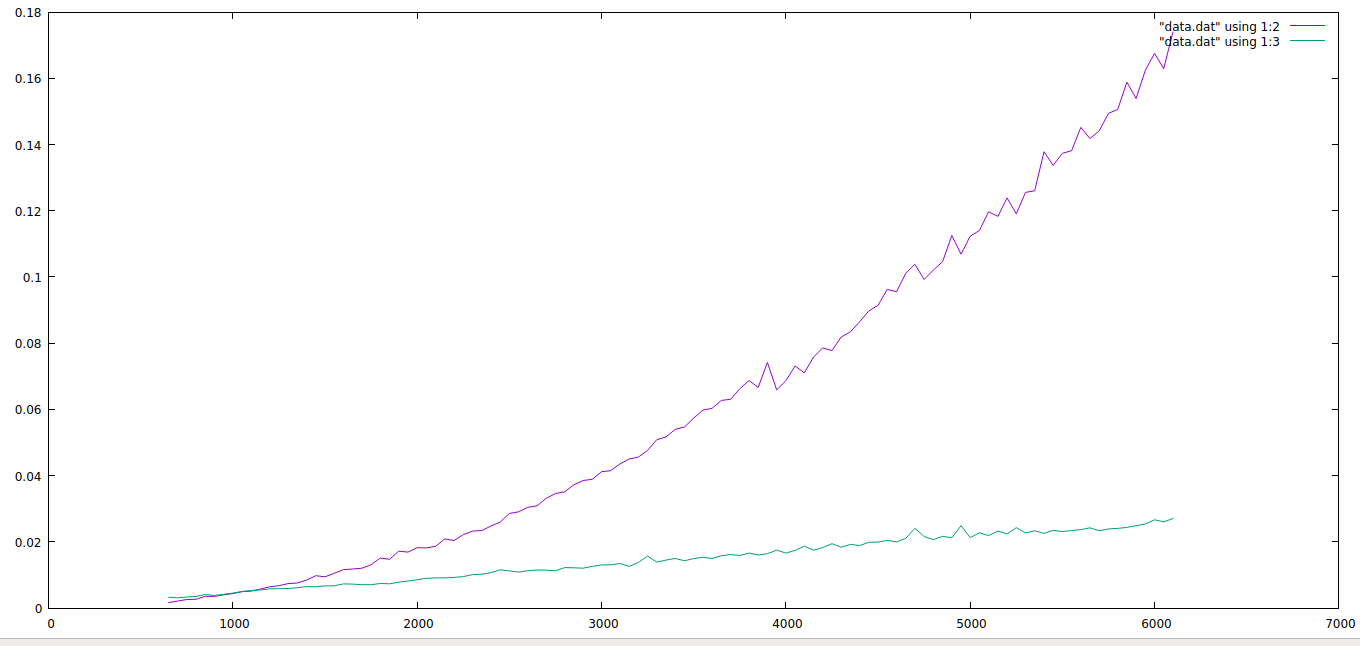
\includegraphics[width=\textwidth]{Src/Gnuplot.png}


Purple: Insertion Sort\\
Green: Mergesort\\

The average is aprox : 1050 n\\
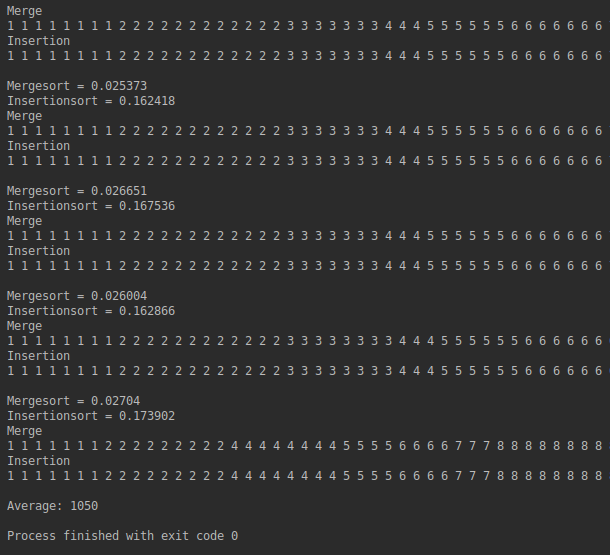
\includegraphics[width=\textwidth]{Src/Average.png}
\section{Research}

Everybody at this point remembers the quadratic ``grade school'' algorithm to multiply 2 numbers of $k_{1}$ and $k_{2}$ digits respectively. \\

Your assignment now is to compare the number of operations performed by the quadratic grade school algorithm and Karatsuba multiplication.

\begin{itemize}
    \item Define Karatsuba multiplication
    \item Implement grade school multiplication
    \item Implement Karatsuba multiplication
    \item Compare Karatsuba algorithm against grade school multiplication
    \item Use any of your implemented algorithms to multiply $a*b$ where:
    \begin{description}
    \item{a:} 3141592653589793238462643383279502884197169399375105820974944592
    \item{b:} 2718281828459045235360287471352662497757247093699959574966967627
    \end{description}
\end{itemize}

Note: Include(.tex) and attach(.cpp) your source code, of course.\\

\emph{BONUS:} How about Sch\"{o}nhage-Strassen algorithm ? 

\begin{lstlisting}[language=C++, caption={Karatsuba}]
#include <iostream>
#include <string>
#include <sstream>
#include <vector>

using namespace std;

string addceros(const string &a, int b, bool lado){
    string respuesta="";
    //si lado es 1 entonces agregara 0s a la derecha
    if(lado==1){
        respuesta=a;
        for(int i=0;i<b;++i)
            respuesta+='0';
    }//caso contrario agregara 0s a la izquierda
    else{
        for(int i=0;i<b;++i)
            respuesta+='0';
        respuesta+=a;
    }
    return respuesta;
}

//Classic
string operator*(const string &a, const string &b){
    string respuesta="";
    int sizea=a.size();
    int sizeb=b.size();
    vector<int> answer(sizea+sizeb,0);
    int puntero,i,j,out,multi,pos=0;
    for (i = sizea-1 ;  i>=0; --i) {
        puntero=pos;
        out=0;
        for(j=sizeb-1 ;j>=0;--j){
            multi=(b[j]-48)*(a[i]-48)+out+answer[puntero];
            if(multi>=10){
                out=multi/10;
                answer[puntero]=multi%10;
            }else{
                out=0;
                answer[puntero]=multi;
            }
            puntero++;
        }
        if(out>0){
            answer[puntero]+=out;
        }
        pos++;
    }
    bool x=true;
    for(int z=answer.size()-1;z>=0;--z){
        if(answer[z]==0 && x )
            continue;
        x=false;
        respuesta+=to_string(answer[z]);
    }
    if(x)
        return respuesta="0";
    return respuesta;
};

string operator-(const string &a,const string &b){
    string respuesta="";
    int sizea=a.size();
    int sizeb=b.size();
    int diferencia=sizea-sizeb;
    string newb=addceros(b,diferencia,0);
    sizeb=newb.size();
    vector<int> answer(sizea,0);
    int i,j,resta,pos=0,out=0;
    for(i=sizea-1;i>=0;--i){
        answer[pos]+=a[i]-48;
        pos++;
    }
    pos=0;
    for(j=sizeb-1;j>=0;--j){
        resta=answer[pos]-(newb[j]-48)-out;
        if(resta<0){
            out=1;
            answer[pos]=10+resta;
        }else{
            out=0;
            answer[pos]=resta;
        }
        pos++;
    }
    bool x=true;
    for(int z=answer.size()-1;z>=0;--z){
        if(answer[z]==0 && x )
            continue;
        x=false;
        respuesta+=to_string(answer[z]);
    }
    if(x)
        return respuesta="0";
    return respuesta;
};

string operator+(const string &a, const string &b){
    string respuesta="";
    int sizea=a.size();
    int sizeb=b.size();

    vector<int> answer(sizea > sizeb  ? sizea+1 : sizeb+1,0);
    int i,j,suma,pos=0,out=0;
    for(i=sizea-1;i>=0;--i){
        answer[pos]+=a[i]-48;
        pos++;
    }
    pos=0;
    for(j=sizeb-1;j>=0;--j){
        suma=(b[j]-48)+answer[pos]+out;
        if(suma>=10){
            out=suma/10;
            answer[pos]=suma%10;
        }else{
            out=0;
            answer[pos]=suma;
        }
        pos++;
    }
    if(out>0)
        answer[pos]+=out;
    bool x=true;
    for(int z=answer.size()-1;z>=0;--z){
        if(answer[z]==0 && x )
            continue;
        x=false;
        respuesta+=to_string(answer[z]);
    }
    if(x)
        return respuesta="0";
    return respuesta;
}

string karatsuba(const string &n1, const string &n2){
    string a,b,c,d,respuesta;
    if(n1.size()==1 || n2.size()==1){
        respuesta=n1*n2;
        return respuesta;
    }
    else{
        string ac,bd,ab,cd,suma,resta, m1,m2,N1,N2;
        int resto=0,size2=0;
        int size = max(n1.size(),n2.size());
        if (size % 2 == 1)
        {
            size = (size + 1) ;
        }
        size2=size/2;
        if(n1.size()<size){
            resto=size-n1.size();
            N1=addceros(n1,resto,0);
        }else{
            N1=n1;
        }
        if(n2.size()<size){
            resto=size-n2.size();
            N2=addceros(n2,resto,0);
        }
        else{
            N2=n2;
        }
        a=N1.substr(0,size2);
        b=N1.substr(size2, size2);
        c=N2.substr(0, size2);
        d=N2.substr(size2, size2);

        ac=karatsuba(a,c);
        bd=karatsuba(b,d);
        ab=a+b;
        cd=c+d;
        suma=karatsuba(ab,cd);
        resta=suma-bd;
        resta=resta-ac;

        m1=addceros(ac,size,1);
        m2=addceros(resta,size2,1);

        respuesta=m1+m2;
        respuesta=respuesta+bd;
    }
    return respuesta;

};

int main() {

    string a="36334570022123324633457902146334579021123161";
    string b="63345730142123324633457901246334579021123232";
    string a1="6351656156315631654514514651465467";
    string b1="6351656156315631621267124651465467";

    string a2="3001233451452561230";
    string b2="3001212332463345790";

    string a3="300221233246334579021";
    string b4="301421233246334579012";

    string a5="36334570022123324633457902146334579021123161";
    string b5="63345730142123324633457901246334579021123232";
    cout<<"Karatsuba"<<endl<<endl;
    clock_t start = clock();
    cout<<karatsuba(a,b)<<endl<<endl;
    cout<<karatsuba(a1,b1)<<endl<<endl;
    cout<<karatsuba(a2,b2)<<endl<<endl;
    cout<<karatsuba(a3,b4)<<endl<<endl;
    cout<<karatsuba(a5,b5)<<endl<<endl;
    clock_t time = clock() - start;
    cout << "Karatsuba time = " << static_cast<float>(time) / CLOCKS_PER_SEC<< endl;

    cout<<"Classic Multiplication"<<endl<<endl;
    start = clock();

    cout<<a*b<<endl<<endl;
    cout<<a1*b1<<endl<<endl;
    cout<<a2*b2<<endl<<endl;
    cout<<a3*b4<<endl<<endl;
    cout<<a5*b5<<endl<<endl;
    time = clock() - start;
    cout << "Third Grade time = " << static_cast<float>(time) / CLOCKS_PER_SEC<< endl;
    cout<<endl<<endl;
    cout<<"A*B Multiplication"<<endl;
    string Teachera="3141592653589793238462643383279502884197169399375105820974944592";
    string Teacherb="2718281828459045235360287471352662497757247093699959574966967627";
    cout<<Teachera*Teacherb<<endl;

    return 0;
}

\end{lstlisting}


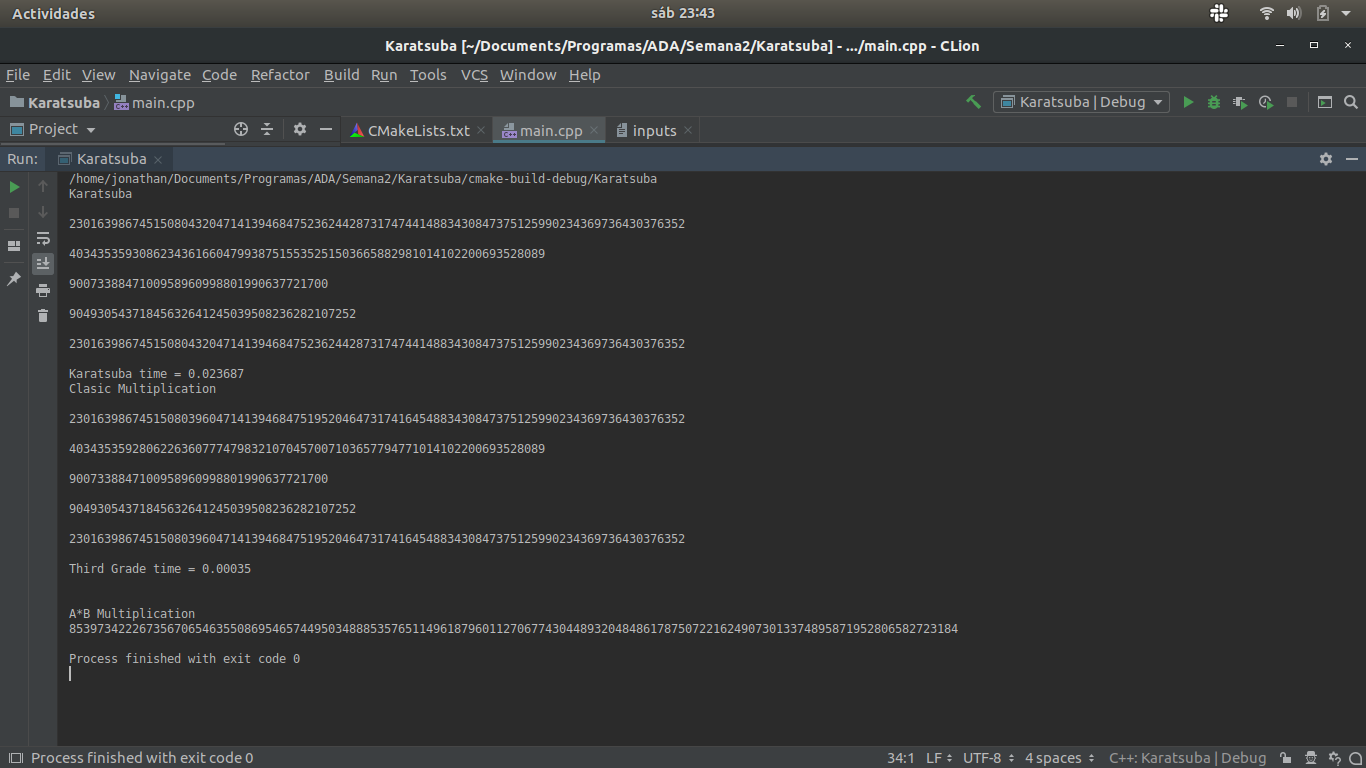
\includegraphics[width=\textwidth]{Src/Pantalla.png}\\

\section{Wrapping up}

Arrange the following functions in increasing order of growth rate with $g(n)$ following $f(n)$ if $f(n) = \mathcal{O}(g(n))$

\begin{enumerate}
    \item $n^{2}log(n)$
    \item $2^{n}$
    \item $2^{2^{n}}$
    \item $n^{log(n)}$
    \item $n^{2}$
\end{enumerate}

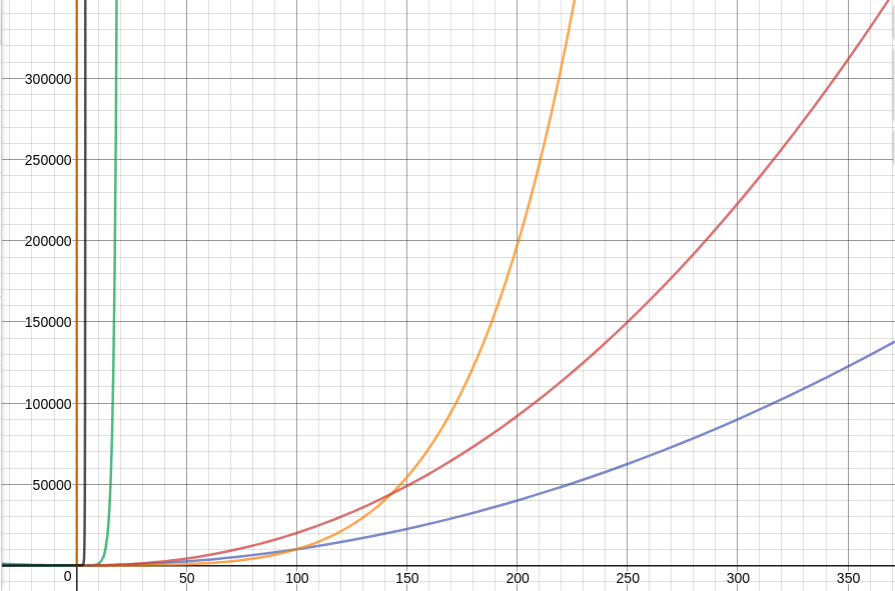
\includegraphics[width=\textwidth]{Src/Grafica5.png}\\

\\The roder of growth is:\\
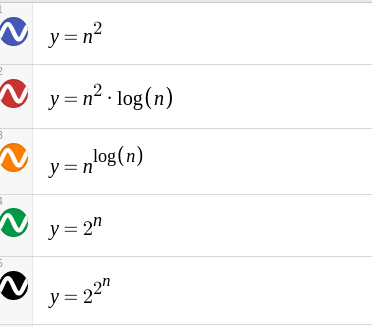
\includegraphics[width=\textwidth]{Src/Leyenda2.png}


\end{document}